\subsection{Block Ciphers}

We use block ciphers to encrypt long (variable input length) messages.
We define a block cipher as a pseudorandom permutation (PRP).
PRP is a pseudorandom function with the constraint that the entries in any two
distinct rows (in a function look-up table) must be different.
A PRP is indistinguishable from a random permutation.
$2^n!$ random permutations exist for $n$ bits. 

Block ciphers have different modes:
\begin{itemize}
    \item Electronic Code Book (ECB)
    \item Cipher Block Chaining (CBC)
    \item Output Feedback (OFB)
    \item Counter (CTR)
\end{itemize}

If we use the electronic code book (ECB) mode of operation
where we chunk the plaintext and apply the block cipher to 
each plaintext block, this isn't even EAV-secure since it's 
deterministic. If a block is repeated in plaintext, 
it will result in a repeating block in the ciphertext.
This could leak a significant amount of information.
Don't use the ECB mode!
\marginnote{Look up "ECB Penguin" for a visual demonstration 
of how insecure ECB is.}

Cipher block chaining, where the plaintext is XORd with 
the ciphertext of the previous block before encryption, 
can be show to be CPA-secure. 

Output feedback, where the 
plaintext is XORd with the ciphertext after encryption, 
is also CPA-secure. In that case the bulk of the computation can be done 
independently of the message.

In counter mode, follow the steps in Figure \ref{fig:ctr}.
\marginnote{Not that kind of nonce.}
\begin{figure}
    \centering
    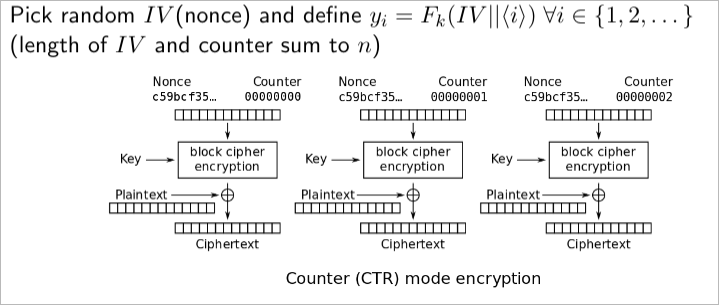
\includegraphics[width=0.9\textwidth]{images/CTR.png}
    \caption{CTR Mode}
    \label{fig:ctr}
\end{figure}

